\documentclass[a4paper,11pt]{article}
\usepackage{graphicx}
\usepackage{subfigure}
\usepackage{amsmath}
\usepackage[pdftex]{hyperref}

\setlength{\textwidth}{16.5cm}
\setlength{\marginparwidth}{1.5cm}
\setlength{\parindent}{0cm}
\setlength{\parskip}{0.15cm}
\setlength{\textheight}{22cm}
\setlength{\oddsidemargin}{0cm}
\setlength{\evensidemargin}{\oddsidemargin}
\setlength{\topmargin}{0cm}
\setlength{\headheight}{0cm}
\setlength{\headsep}{0cm}

\renewcommand{\familydefault}{\sfdefault}

\graphicspath{{pics/}}




\title{Data Mining: Learning From Large Data Sets\\\vspace{2mm}\Large{Fall Semester 2015}}
\author{\{usamuel, adavidso, kurmannn\}@student.ethz.ch}
\date{\today}

\begin{document}
\maketitle
\thispagestyle{empty}
\pagestyle{empty}

\section{Approximate near-duplicate search using Locality Sensitive Hashing}

\paragraph{Problem formulation.\!\!\!}
This project concerned the detection of near-duplicate videos using Locality Sensitive Hashing. The data consisted of sets of shingles for the different videos, and the goal was to find all pairs of videos that had a Jaccard similarity of at least $90$ percent.

\paragraph{Approach.\!\!\!}
To solve the task, we applied the algorithm outlined in the lecture on near-duplicate detection using LSH. First, the signature vector $S_i$ for each document $C_i$ is computed. The resulting signature matrix is then split into $b$ bands, each band having $r$ rows. 
Every column in every band is then hashed, and two documents are considered as potentially similar if they hash into the same bucket for at least one band. Verification of similarity is performed by calculating the actual Jaccard similarity. Our implementation relies on the MapReduce model.

\paragraph{Mapper.\!\!\!}
The mapper processes one document at a time. After having extracted its id and set of shingles, it first computes the signature vector $S_i$ by using $b\cdot r$ randomly generated min-hash functions. Each min-hash function is generated by choosing two integers $a, b \in [1,10000]$ uniformly at random. These two numbers are then used to construct a pseudorandom permutation $\pi(x) = x \cdot a + b\ \operatorname{mod}\ N,$ where $N$ is the size of the shingle vector ($20000$). 
The signature vector is then divided into $b$ bands, each of which is hashed with a random linear hash function. 
A linear hash function is generated by choosing 
$a_1,\dots,a_r,b \in [1,10000]$ uniformly at random. A band is then hashed as follows: $h(s_1,\dots, s_r) = \sum_{i=1}^r a_i s_i + b$.
We used the Python \texttt{int} data type to compute all values, because it gives us an implicit modulo operator due to integer overflow. 
It would have been possible to reuse the same linear hash function for each band because we never compare the hash values of two different bands. 
However we decided to use multiple hash functions because this follows the approach that was presented in the lecture more closely.

For each video and each band, the mapper then emits the following key-value pair: $$\text{key}=\text{(band id, hash value of band)},\enspace\text{value}=(\text{video id, vector of shingles}).$$

\paragraph{Reducer.\!\!\!}
The MapReduce framework groups all emitted key-value pairs by key and passes them to the reducer. 
This means that all videos that hash to the same bucket in a band (candidate pairs) are grouped together. 
The reducer then only has to report these candidate pairs.
However, since a pair of videos may hash to the same bucket in multiple bands, we had to account for duplicates and print each candidate pair only once. 
We solved this issue by keeping track of all pairs that had been printed in a hash table. 
Before printing a new pair, we first checked in this table to see whether the pair already had been reported or not.

This approach yielded a precision of around $0.5$.
We boosted our precision by letting the reducer compute the actual Jaccard similarity between two potential near-duplicates, thus eliminating false positives. 
This is why we had the mapper emit the vector of shingles associated with a given video in addition to the video id. 

\paragraph{Results.\!\!\!}
Using $28$ bands and $35$ rows, see Figure \ref{fig:a}, resulted in a precision of $1.0$ and a recall value of $0.994$. In order to have the recall also attain a value of $1.0$, we needed to eliminate the remaining false negatives. Thus, we shifted the S-curve slightly to the left by instead using $50$ bands and $20$ rows, see Figure \ref{fig:b}, which resulted in both precision and recall attaining the value of $1.0$. The drawback of this shift was that it increased the number of false positives, and so the reducer had to do some more work using these parameter values.

\paragraph{Workload distribution.\!\!\!}
A working implementation of the algorithm including the hash functions was created by Sam. As a group, we then chose to eliminate the false positives by computing the exact Jaccard distance, after which we tweaked the number of bands and rows per band, using plots provided by Alexander. A minimalist draft of the report was created as a group, but was then fleshed out by Sam and Alexander. This overview of the workload distribution was provided by Nico.



\begin{figure}[t]
\centering
\subfigure[$28$ bands, $35$ rows.]{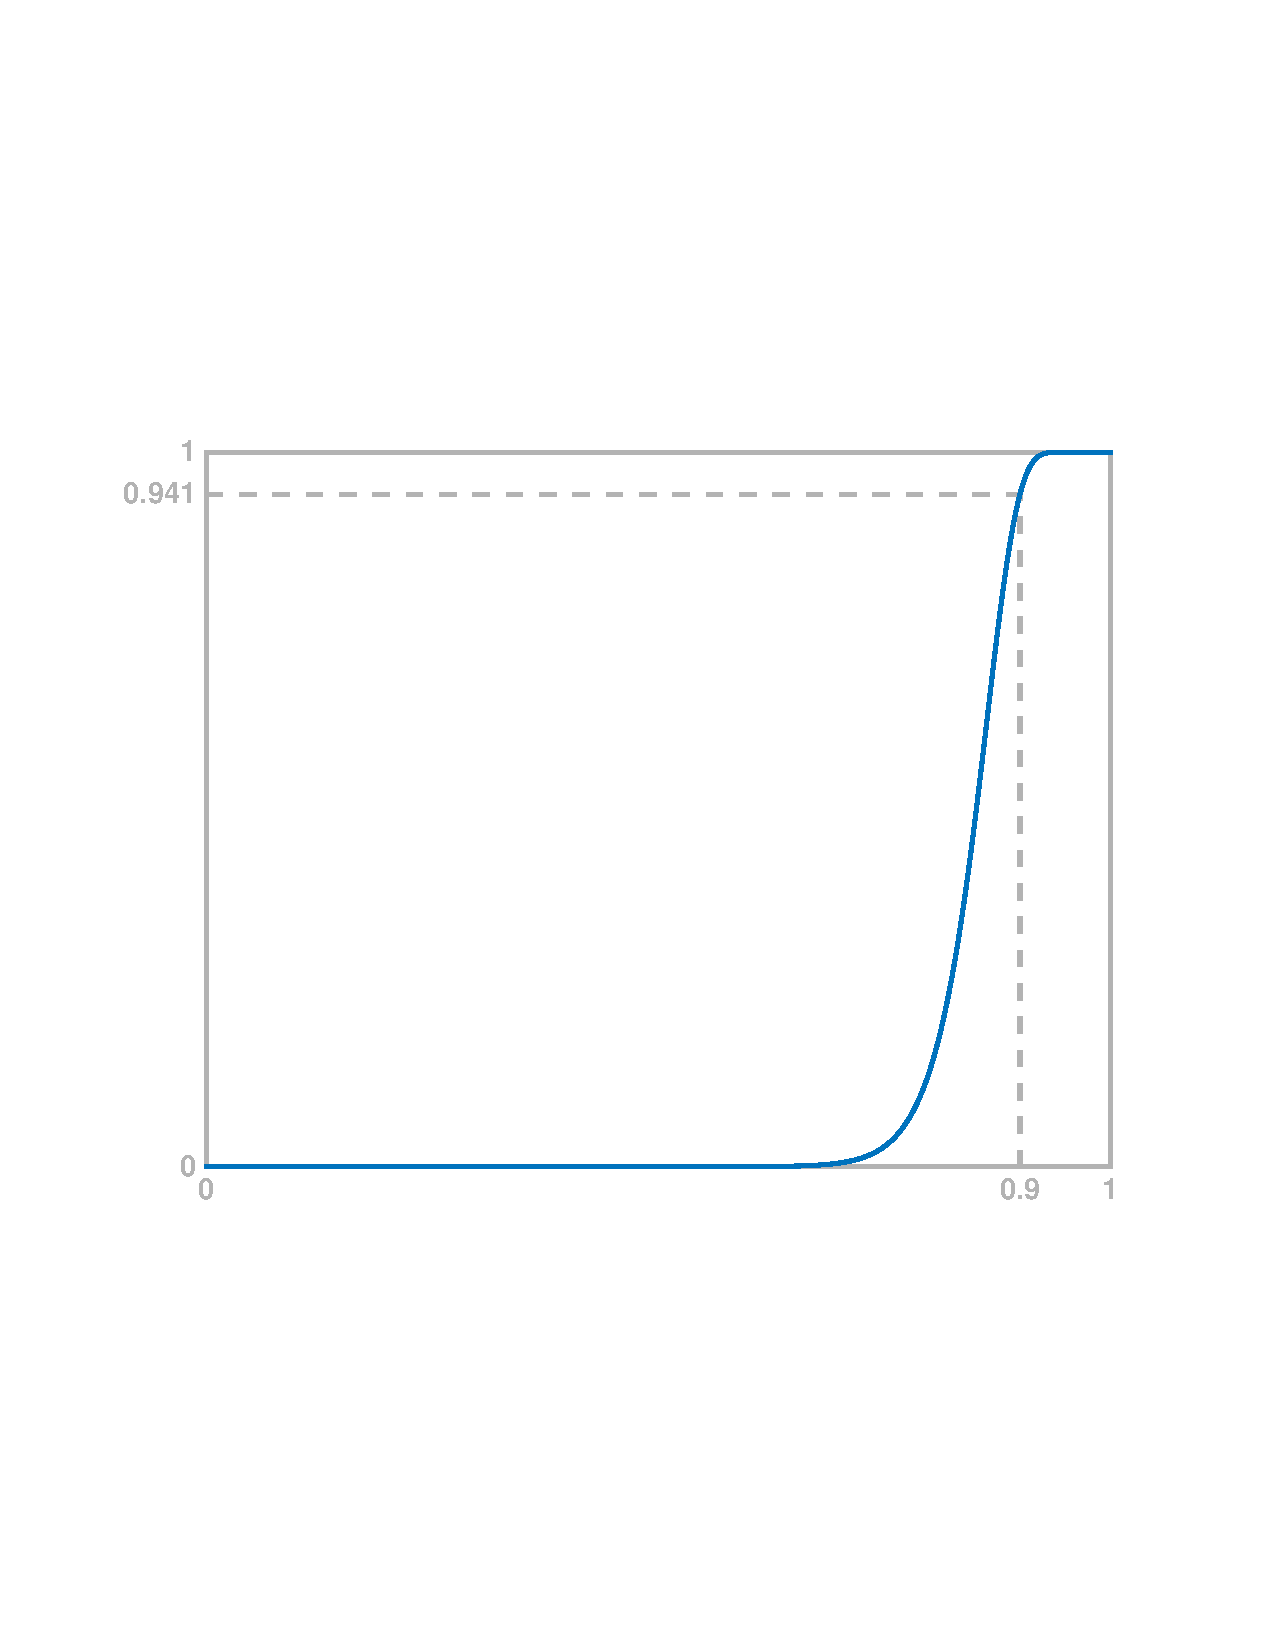
\includegraphics[trim=17mm 73mm 17mm 72mm,clip=true,scale=0.1,width=.48\textwidth]{curve.pdf}\label{fig:a}}
\subfigure[$50$ bands, $20$ rows.]{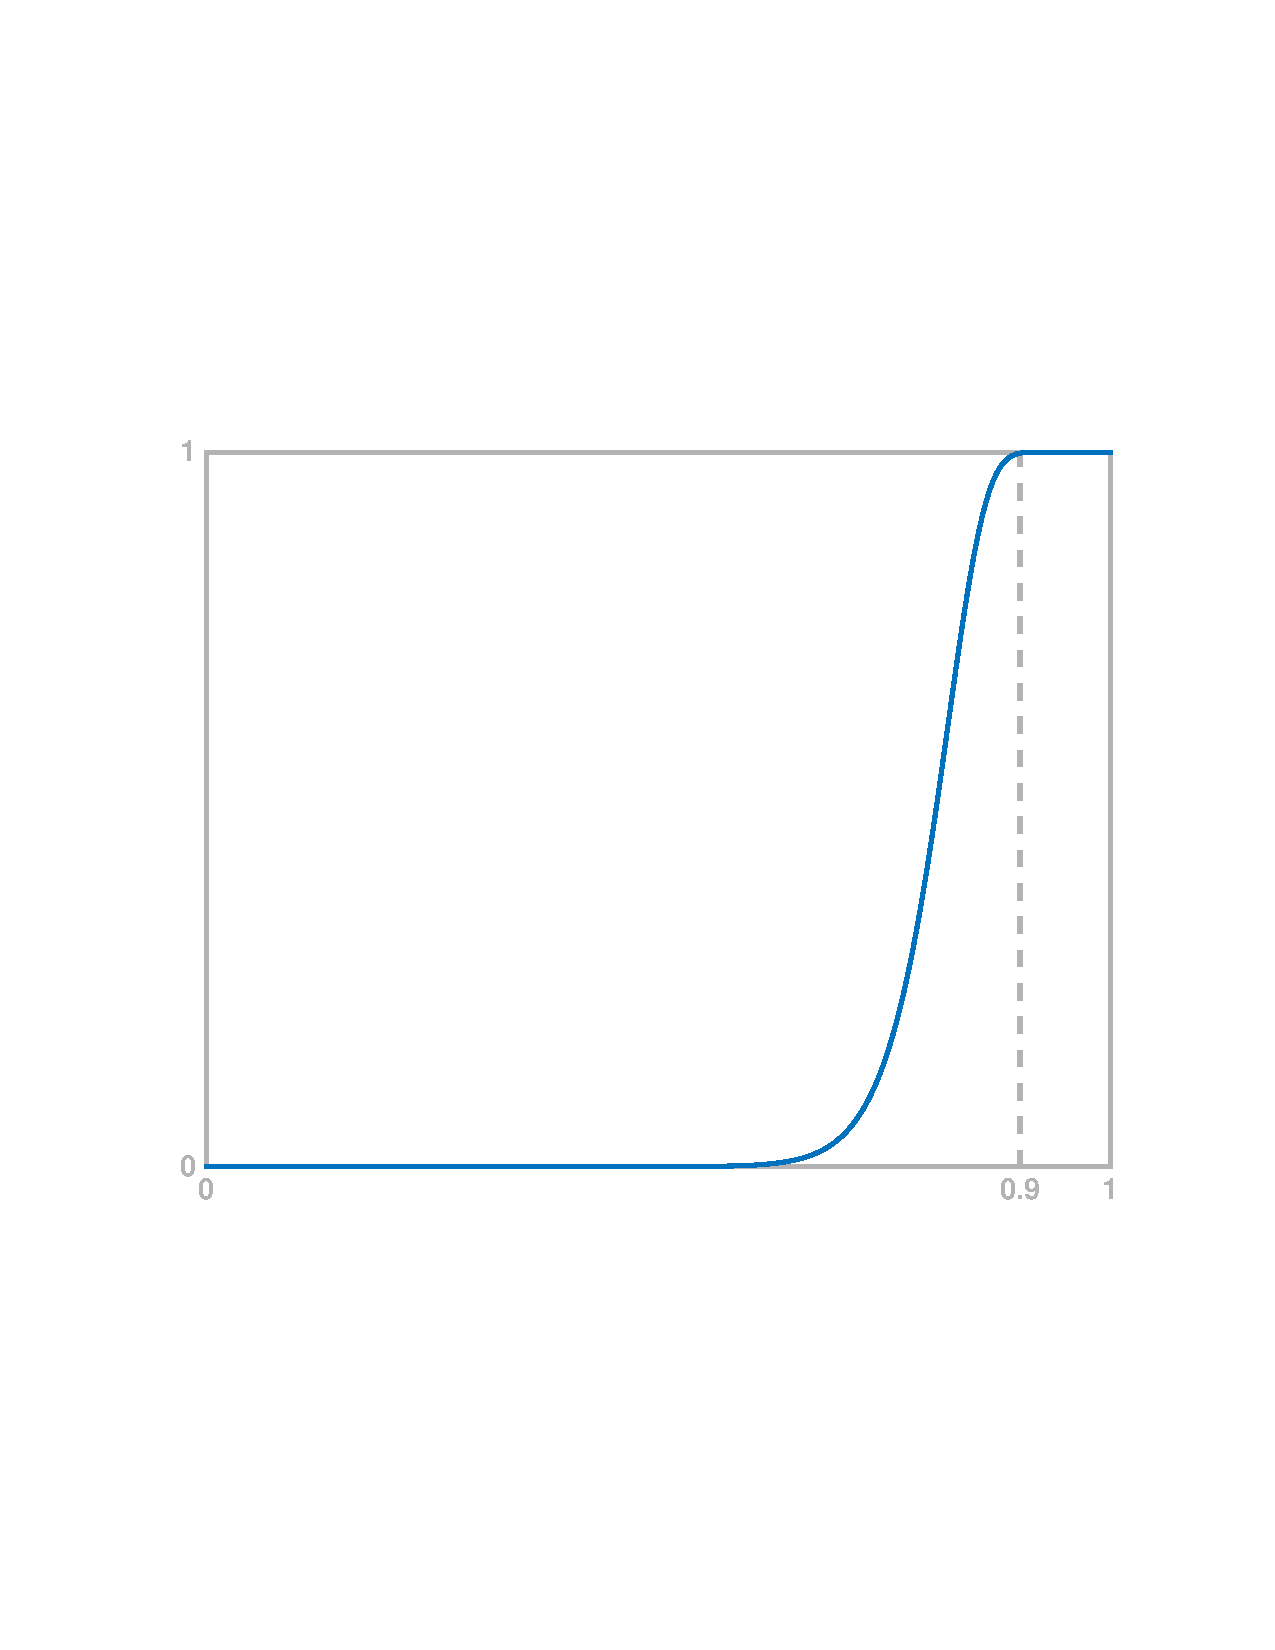
\includegraphics[trim=17mm 73mm 17mm 72mm,clip=true,scale=0.1,width=.48\textwidth]{curve3.pdf}\label{fig:b}}
\caption{S-curves for our different combinations of parameter values.}
\label{fig:wifi}
\end{figure}


% -----------------------------------------

\newpage
\section{Large Scale Image Classification} 

% \texttt{Briefly describe the steps used to produce the solution. Feel free to add plots or screenshots if you think it's necessary. The report should contain a maximum of 2 pages.
% Keep in mind that you only have to submit one report per group. Please indicate the contribution of each group member to the project.}

\paragraph{Problem formulation.\!\!\!}
The goal of this project was to construct an SVM that classifies images into one of two classes, these classes being images of people versus images of nature. The images were provided in the form of precomputed feature vectors, each containing $400$ features.

\paragraph{Approach and Results.\!\!\!}
We constructed a classifier by running SGD in each mapper. Each mapper reads values $(y_t,x_t)$, for $1\leq t\leq T$, and then computes $w_t$ using the SGD algorithm, as presented in class. The final result of the mapper is the average of
all $w_t$. The reducer collects and averages over these hyperplanes, and outputs the final classifier $w$.

We tried several approaches to compute a good classifier for the image classification problem.

At first, we used OCP to compute a linear classifier. The features were used ``as is" with the addition of a constant $1$ to account for an intercept. We chose $\eta_t=1/\sqrt{t}$ and $\lambda=1$. This approach yielded a score of about $60$ percent.

To improve on this, we tried to process the feature vectors in random order, as is done in SGD. We adapted the mapper to first store the entire input in a matrix. This matrix was then processed uniformly at random. To make the most out of the available computation time, we kept on reading from the matrix in random order for around $4.5$ minutes. In addition, we chose $\lambda=1/N$, with $N$ being the number of feature vectors passed to the mapper, and $\eta= 1/(\lambda t)$. 
This approach yielded a score of approximately 70 percent.

We were not able to improve on this and therefore assumed that the feature vectors were not (sufficiently)
linearly separable. We experimented with several non-linear feature transformations, and were able to boost our score to 81 percent with the following transformation, which uses built-in NumPy functions:
\begin{equation*}
\texttt{x <- [numpy.sqrt(x), numpy.diff(x), numpy.gradient(x)]}.
\end{equation*}
This might seem like an odd transformation, but the motivation for doing this was that the original feature vectors were sparse, and so we wanted to remove some of this sparsity, which is why we use \texttt{diff} and \texttt{gradient}.

Finally, we were able to beat the hard baseline by using random Fourier features on top of the above transformed features. Sampling 3,500 of these resulted in a score of 84 percent. At this point in time, we noticed that the first entry in every original feature vector in the training set was zero, so we dropped this feature.

\paragraph{Workload distribution.\!\!\!}
Nico and Alexander wrote the initial structure for the mapper and reducer. Samuel implemented the basic OCP algorithm. Alexander extended this to include SGD and he also came up with the non-linear transformations. Samuel implemented random Fourier features (with errors), and Alexander corrected the errors, which then resulted in our final mapper. Everybody contributed to the report.



% -----------------------------------------

\newpage
\section{Extracting Representative Elements} 

\paragraph{Problem formulation.\!\!\!}

Given a set of features of images that belong to different (unknown) clusters, the goal was to find representative elements for each cluster. The quality of our selection is quantified by the sum of quadratic distances that each representative has to the elements of its cluster.
This problem statement is equivalent to the solution of k-means, but we were able to use a map-reduce framework to speed up this process.


\paragraph{Approach and Results.\!\!\!}

To solve this problem, we used SciKit Learn's integrated implementation of kmeans, which internally uses kmeans++ to generate good starting centers that help the algorithm converge faster.

In our initial approach, we ran kmeans on the mappers to compute k=200 centers each, which were then all passed to the reducer, who in turn ran kmeans to reduce the number of centers to 100, which we then proceeded to output as our result. Increasing the number of centers computed by the mappers to 1000 gave us the surprisingly high score of 9.17742.

This was without taking into the consideration the weights of the clusters/coresets passed by the mappers. We tried to override SciPy's kmeans update centers method, but we failed because it is defined in the binary file \verb|_k_means.x86_64-linux-gnu.so|. Another approach was to adapt the mapper to output each center multiple times proportionally to its weight. However, this approach didn't improve our score.

In our third approach, we kept the mappers mostly the same, but we tried to take into account the weights of the centers outputted by the mappers. For this, we stopped performing kmeans in the reduce step, but instead opted for merging the points manually. For this, the reducer selected a random center and merged it with the closest other center by taking a weighted average.
This approach netted us with a score of 9.02585.


\paragraph{Workload distribution.\!\!\!}

Alexander implemented the initial approach. At first there were some technical problems that caused his code to crash on the cluster. This issue was
resolved by Samuel. The entire group then tried to optimize the parameters of the first approach and discussed other approaches. Nico tried to overwrite 
SciKits internal kmeans implementation. Samuel adapted the initial solution to output centers multiple times. 
Alexander implemented the final approach where the reducer merges the centers. Nico wrote the final report.


% -----------------------------------------

\newpage
\section{Explore-Exploit tradeoffs in Recommender Systems} 

\paragraph{Problem formulation.\!\!\!}
The goal of this project was to implement an algorithm that solves the contextual k-armed bandits problem. 
This algorithm should recommend news article to a user based on that users preferences.

\paragraph{Approach and Results.\!\!\!}

Our first attempt was to implement the LinUCB algorithm as it was presented in the lecture. 
At first, our implementation of LinUCB would not terminate within the given 15 minutes on the cluster. 
We figured out that the computational complexity was dominated by the linear system of equations that had to be solved 
for each article in each recommendation step. In the end, we were able to come up with a faster implementation by using
the Sherman-Morrison formula\footnote{http://en.wikipedia.org/wiki/Sherman-Morrison\_formula}:
$$(A+uv^T)^{-1} = A^{-1} - {A^{-1}uv^T A^{-1} \over 1 + v^T A^{-1}u}$$

We changed our algorithm to store the inverse of the $M_x$ matrix for each article instead of just $M_x$. By doing so we no longer had to 
solve a system of equations in each round. The Sherman-Morrison formula allowed us to efficiently update this inverse matrix. 
This change dramatically increased the performance of our implementation and it ran in approximately 12 minutes on the cluster.
\\\\
The next thing we did was to find an optimal value for $\alpha$. 
We ran our algorithm with several different values between $3$ and $0.1$ (see figure \ref{fig:scores}). 
With $\alpha=0.3$ we got the highest score of 0.065674.
\\\\
In addition to LinUCB we also tried several other approaches. We tried UCB1 and Thompson sampling which both scored lower than LinUCB. 
We also tried to do a non-linear transformation of the user features by using random fourier features. 
Unfortunately this version of our algorithm would not terminate on the cluster.
Another approach we tried was to combine the user vector with the article vector in LinUCB as it is mentioned in the original paper. This however
would not result in a better score than our original LinUCB implementation.

\begin{figure}[t]
\centering
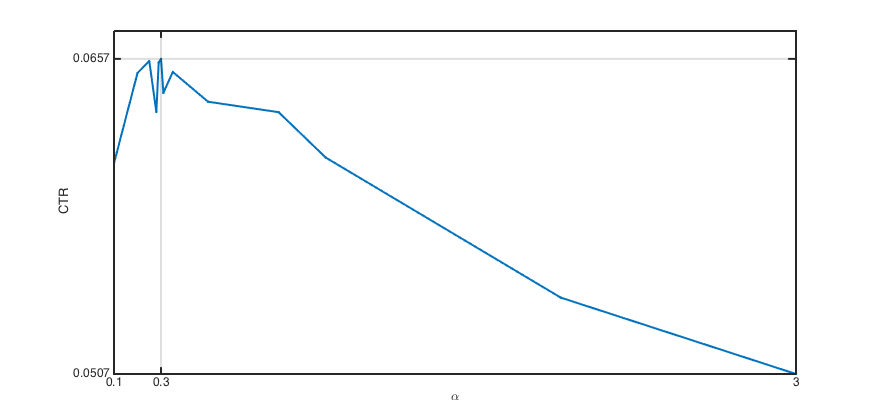
\includegraphics[width=0.8\textwidth]{scores}
\caption{Score of LinUCB with different values for $\alpha$.}
\label{fig:scores}
\end{figure}

\paragraph{Workload distribution.\!\!\!}

Samuel wrote the first implementation of LinUCB and UCB1 and he came up with the idea to use the Sherman-Morrison formula.
Alexander adapted the LinUCB implementation to the Sherman-Morrison formula. 
Alexander tried out Thompson sampling and combining the user vector with the article vector. 
Samuel tried out random fourier features. Nico wrote a draft of the report and Samuel finished it.

\end{document}
